\newpage
\section{Element library}
\label{section:ElementLibrary}
\subsection{PML elements}

\emph{Perfectly matched layers} (PMLs) are what is used to model
the effect of energy loss through supports or anchor loss.
PMLs mimic the effect of an infinite or semi-infinite medium,
by applying complex-value coordinate transformations.
PMLs fit naturally
into a finite element framework, but to implement them, we need some
way to describe the exact form of the coordinate transformation.
This coordinate-stretching function used in a PML is is defined as a
Lua function and set to the set to the element that
the PML is imposed by the following function:
\begin{codelist}

  \item[set\_stretch(stretch\_func)]
    Use a Lua function \ttt{stretch\_func} to describe the coordinate 
    transformation.  
    The coordinate stretching function in 2D should have the form
    \begin{verbatim}
  function stretch_func(x,y)
    -- Compute stretching parameters sx and sy
    return sx, sy
  end
    \end{verbatim}
    If no stretch values are returned, they are assumed to be zero.
    The PML element should stretch the $x$ and $y$ coordinates by
    $(1-is_x)$ and $(1-is_y)$, respectively.  The 3D case is handled
    similarly.

    This function is set to the element in the following manner.
    \begin{verbatim}
  element_to_apply_pml:set_stretch(stretch_func)
    \end{verbatim}

    The stretching function is only ever evaluated at node positions.

\end{codelist}
If there are no calls to either form of \ttt{set\_stretch}, the PML
element does not stretch the spatial coordinate at all, and so the
element behaves exactly like an ordinary (non-PML) element.

For the exact form of this coordinate transformation function and
details in implementation, see the PML example in the Examples
Manual.

\clearpage
\subsection{Laplace elements}

The \ttt{PMLScalar1d}, \ttt{PMLScalar2d}, \ttt{PMLScalar3d}, 
and \ttt{PMLScalarAxis}
classes implement scalar wave equation elements with an optional PML.
The general constructor takes the form,
\begin{codelist}
  \item[etype = make\_material\_s(mtype,analysistype)]
\end{codelist}
The variable \ttt{mtype} must contain the fields
\ttt{rho}(mass density) and \ttt{E}(material stiffness).
The variable \ttt{analysis\_type} can take one of the 
following strings,
\begin{itemize}
\item \ttt{1d}: 1 dimensional analysis
\item \ttt{2d}: 2 dimensional analysis
\item \ttt{3d}: 3 dimensional analysis
\item \ttt{axis}: Axis symmetric analysis
\end{itemize}
The scalar wave equation has the form,
\begin{eqnarray}
\rho \frac{\del^2 u}{\del t^2} &=& 
              \bfnabla\cdot \left( \bkappa \bfnabla u \right)
\end{eqnarray}
where $u$ is the scalar displacement, $\rho$ is the density, 
and $\bkappa$ is the stiffness. 
If no coordinate stretching is 
defined, the elements will generate standard (real) mass and 
stiffness matrices.
The class provides the following constructors:

\begin{codelist}

  \item[PMLScalar1d(kappa,rho)] 
    Creates an isotropic 1D scalar wave equation element with material
    property $\kappa$ and mass density $\rho$.  

  \item[PMLScalar2d(kappa,rho)] 
    Creates an isotropic 2D scalar wave equation element with material
    property $\kappa$ and mass density $\rho$. 

  \item[PMLScalar2d(D,rho)]
    Creates a 2D anisotropic element with a 2-by-2 property matrix
    \ttt{D}.  Other than the material properties, this constructor is
    identical to the previous one.

  \item[PMLScalarAxis(kappa,rho)]
    Creates an isotropic axisymmetric scalar wave equation element
    with material property $\kappa$ and mass density $\rho$.  

  \item[PMLElasticAxis(D,rho)]
    Creates a 2D anisotropic element with a 2-by-2 property matrix
    \ttt{D}.  Other than the material properties, this constructor is
    identical to the previous one.

  \item[PMLScalar3d(kappa,rho)] 
    Creates an isotropic 3D scalar wave equation element with material
    property $\kappa$ and mass density $\rho$.  

  \item[PMLScalar3d(D,rho)]
    Creates a 3D anisotropic element with a 3-by-3 property matrix
    \ttt{D}.  Other than the material properties, this constructor is
    identical to the previous one.

\end{codelist}

\clearpage
\subsection{Elastic elements}

The \ttt{PMLElastic2d}, \ttt{PMLElastic3d}, and \ttt{PMLElasticAxis}
classes implement elasticity (Solid) elements with an optional PML
transformation. 
The general constructor takes the form,
\begin{codelist}
  \item[etype = make\_material\_e(mtype,analysistype)]
  \item[etype = make\_material\_e(mtype, etype, wafer, angle)]
    Constructs and returns a \ttt{PMLElastic} element, depending on the
    given arguments. The material type \ttt{mtype} (string or table containing
    material mechanical properties) and element type
    \ttt{etype}(\ttt{planestrain,planestress,axis,3d}) must be given. 
    The arguments defining wafer orientation \ttt{wafer}(\ttt{'100'} or
    \ttt{'111'}) and orientation angle \ttt{angle} [rad] are optional.
    The table of mechanical properties \ttt{mtype} should contain the 
    fields \ttt{rho, E, nu} for isotropic material, and \ttt{lambda, mu,
    alpha} for cubic material.
    (Currently this element can only treat cubic and isotropic mechanical
     material).
\end{codelist}
The variable \ttt{mtype} must be an elastic materail containing
different fields depending on the symmetry of the crystal considered.
In the case of anisotropic material the second constructor is used,
which defines the wafer orientation and angle.
The variable \ttt{analysis\_type} can take one of the 
following strings,
\begin{itemize}
\item \ttt{planestrain}: 2 dimensional planestrain analysis
\item \ttt{planestress}: 2 dimensional planestress analysis
\item \ttt{3d}: 3 dimensional analysis
\item \ttt{axis}: Axis symmetric analysis
\end{itemize}
These elements solve the following equation,
\begin{eqnarray}
\rho \frac{\del^2 \bfu}{\del t^2}
&=& \bfnabla\cdot\bsig \\
\bsig &=& \bbC:\beps \\
\beps &=& \bfnabla_\text{sym}\bfu
\end{eqnarray}
Here, $\rho$ is the density, $\bsig$ is the stress, $\bbC$ is the
material stiffness tensor, $\beps$ is the infinitesimal strain, and
$\bfu$ is the displacement vector. In the case of an isotropic material,
$\bbC$ will depend only on two variables: the Youngs modulus $E$ and 
Poisson ratio $\nu$. Otherwise the material property can be expressed
by a matrix via Voigt notation. (See section on material models for
further information).
 If no coordinate stretching is 
defined, the elements will generate standard (real) mass and 
stiffness matrices.
The classes provides the following constructors:
\begin{codelist}

  \item[PMLElastic2d(E,nu,rho,plane\_type)]
    Creates a plane strain (\ttt{plane\_type = 0}) or plane stress
    (\ttt{plane\_type = 1}) isotropic elasticity element with
    Young's modulus \ttt{E}, Poisson ratio \ttt{nu}, and mass
    density \ttt{rho}.  

  \item[PMLElastic2d(D,rho)]
    Creates a 2D element with a 3-by-3 elastic property matrix
    \ttt{D}.  Other than the elastic properties, this constructor
    is identical to the previous one.

  \item[PMLElastic2d(lua\_State* L, lua\_Object func)]
    Creates a 2D element with material parameters defined by a
    Lua function \ttt{func}. This function is accessed via the 
    Lua state \ttt{L}. \ttt{func} must take one of the following
    forms. 
    \begin{verbatim}
  function material_function(x,y)
    -- Compute 3-by-3 elastic property matrix D and 
    --                mass density rho
    return D, rho
  end
    \end{verbatim}
    or,
    \begin{verbatim}
  function material_function(x,y)
    -- Compute Young's modulus E, Poisson ration nu, 
    --         mass density rho, and analysis plane_type
    return E, nu, rho, plane_type
  end
    \end{verbatim}
  
  \item[PMLElasticAxis(E,nu,rho)]
    Creates an isotropic axisymmetric elasticity element with
    Young's modulus \ttt{E}, Poisson ratio \ttt{nu}, and mass
    density \ttt{rho}.  

  \item[PMLElasticAxis(D,rho)]
    Creates an element with a 4-by-4 elastic property matrix
    \ttt{D}.  Other than the elastic properties, this constructor
    is identical to the previous one.

  \item[PMLElasticTAxis(E,nu,rho,ltheta)]
    Creates an isotropic axisymmetric elasticity element with
    Young's modulus \ttt{E}, Poisson ratio \ttt{nu}, mass
    density \ttt{rho}, and wave number \ttt{ltheta}.

  \item[PMLElasticTAxis(D,rho,ltheta)]
    Creates an element with a 6-by-6(????) elastic property matrix
    \ttt{D}.  Other than the elastic properties, this constructor
    is identical to the previous one.

  \item[PMLElastic3d(E,nu,rho)] 
    Creates an isotropic 3D elasticity element with Young's modulus
    \ttt{E}, Poisson ratio \ttt{nu}, and mass density
    \ttt{rho}.  

  \item[PMLElastic3d(D,rho)]
    Creates an element with a 6-by-6 elastic property matrix
    \ttt{D}.  Other than the elastic properties, this constructor
    is identical to the previous one.

\end{codelist}

\clearpage
\subsection{Thermoelastic Elements}

The \ttt{PMLElastic2d\_te}, \ttt{PMLElastic3d\_te}, 
and \ttt{PMLElasticAxis\_te}
classes implement thermoelasticity (Solid) elements with an optional PML
transformation. 
The general constructor takes the form,
\begin{codelist}
  \item[etype = make\_material\_te(mtype,analysistype)]
  \item[etype = make\_material\_te(mtype,analysistype,wafer,angle)]
    Constructs and returns a \ttt{PMLElastic\_te} element, depending on the
    given arguments. The material type \ttt{mtype} (string or table containing
    material thermomechanical properties) and element type
    \ttt{etype}(\ttt{planestrain,planestress,axis,3d}) must be given. 
    The arguments defining wafer orientation \ttt{wafer}(\ttt{'100'} or
    \ttt{'111'}) and orientation angle \ttt{angle} [rad] are optional.
    The table of thermomechanical properties \ttt{mtype} should contain the 
    fields \ttt{rho, E, nu} for isotropic material, and \ttt{lambda, mu,
    alpha} for cubic material. For both cases it should contain the fields
    \ttt{at, cp, kt} and \ttt{T0}.
    (Currently this element can only treat cubic and isotropic thermomechanical
     material).
\end{codelist}
The variable \ttt{mtype} must be an elastic materail containing
different fields depending on the symmetry of the crystal considered.
In the case of anisotropic material the second constructor is used,
which defines the wafer orientation and angle.
The variable \ttt{analysis\_type} can take one of the 
following strings,
\begin{itemize}
\item \ttt{planestrain}: 2 dimensional planestrain analysis
\item \ttt{planestress}: 2 dimensional planestress analysis
\item \ttt{3d}: 3 dimensional analysis
\item \ttt{axis}: Axis symmetric analysis
\end{itemize}
These elements solve the following coupled equation,
\begin{eqnarray}
\rho \frac{\del^2 \bfu}{\del t^2}
&=& \bfnabla\cdot\bsig \\
\rho c_v \dot{\theta} 
&=& \bfnabla\cdot\left(\bkappa_T\bfnabla \theta\right)
   - T_0 \dot{\beps}:\bbC:\balpha_T\\
\bsig &=& \bbC:\left(\beps - \balpha_T \theta \right)\\
\beps &=& \bfnabla_\text{sym}\bfu
\end{eqnarray}
Here, $\rho$ is the density, $\bsig$ is the stress, $\bbC$ is the
material stiffness tensor, $\beps$ is the infinitesimal strain, 
$\bfu$ is the displacement vector and $\theta$ is the temperature
fluctuation from $T_0$, which is the referential temperature.
In the case of an isotropic material,
$\bbC$ will depend only on two variables: the Youngs modulus $E$ and 
Poisson ratio $\nu$. In the case of a cubic material, it will depend
on three variables: $\lambda$, $\mu$, and $\alpha$.  In both cases 
the material property can be expressed by a matrix via Voigt notation. 
(See section on material models for further information). The constants
related with the thermal field are, $\bkappa_T$ the thermal conductivity
tensor, $c_v$ the specific heat at constant volume, and $\balpha_T$ which
is the linear coefficient of thermal expansion tensor. 
If no coordinate stretching is defined, the elements will generate 
standard (real) mass and stiffness matrices.
The classes provides the following constructors:
\begin{codelist}
  \item[PMLElastic2d\_te(E,nu,rho,at,cp,kt,T0,plane\_type)]
    Creates a plane strain (\ttt{plane\_type = 0}) or plane stress
    (\ttt{plane\_type = 1}) isotropic thermoelasticity element with
    Young's modulus \ttt{E}, Poisson ratio \ttt{nu}, mass
    density \ttt{rho}, coefficient of thermal expansion \ttt{at},
    thermal capacity at constant pressure \ttt{cp}, thermal conductivity
    at \ttt{kt}, and reference temperature \ttt{T0}.

  \item[PMLElastic2d\_te(Db,rho,at,cp,kt,T0)]
    Creates a 2D element with a 4-by-4 thermoelastic property matrix
    \ttt{D}.  Other than the thermoelastic properties, this constructor
    is identical to the previous one.

  \item[PMLElastic3d\_te(E,nu,rho,at,cp,kt,T0)]
    Creates an isotropic 3D thermoelasticity element with Young's modulus
    \ttt{E}, Poisson ratio \ttt{nu}, mass density \ttt{rho},
    coefficient of thermal expansion \ttt{at},
    thermal capacity at constant pressure \ttt{cp}, thermal conductivity
    at \ttt{kt}, and reference temperature \ttt{T0}.

  \item[PMLElastic3d\_te(Db,rho,at,cp,kt,T0)]
    Creates a 3D element with a 7-by-7 thermoelastic property matrix
    \ttt{D}.  Other than the thermoelastic properties, this constructor
    is identical to the previous one.

  \item[PMLElasticAxis\_te(E,nu,rho,at,cp,kt,T0)]
    Creates an isotropic axisymmetric elasticity element with
    Young's modulus \ttt{E}, Poisson ratio \ttt{nu}, mass density \ttt{rho},
    coefficient of thermal expansion \ttt{at},
    thermal capacity at constant pressure \ttt{cp}, thermal conductivity
    at \ttt{kt}, and reference temperature \ttt{T0}.

  \item[PMLElasticAxis\_te(Db,rho,at,cp,kt,T0)]
    Creates an element with a 5-by-5 thermoelastic property matrix
    \ttt{D}.  Other than the thermoelastic properties, this constructor
    is identical to the previous one.
\end{codelist}

\clearpage
\subsection{Piezoelectric elements}
The \ttt{PMLElastic2d\_pz}, \ttt{PMLElastic3d\_pz}, 
and \ttt{PMLElasticAxis\_pz}
classes implement piezoelectric elasticity (Solid) elements with an 
optional PML transformation. 
The general constructor takes the form,
\begin{codelist}
  \item[etype = make\_material\_pz(mtype,analysistype)]
  \item[etype = make\_material\_pz(mtype,analysistype,wafer,angle)]
    Constructs and returns a \ttt{PMLElastic\_pz} element, depending on the
    given arguments. The material type \ttt{mtype} (string or table containing
    material thermomechanical properties) and element type
    \ttt{etype}(\ttt{planestrain,planestress,2hd,3d}) must be given. 
    The arguments defining wafer orientation \ttt{wafer}(\ttt{'100'} or
    \ttt{'111'}) and orientation angle \ttt{angle} [rad] are optional.
    The table of thermomechanical properties \ttt{mtype} should contain the 
    fields \ttt{c11, c12, c13, c33, c55, d16, d31, d33, kds1, kds3} for a 
    hexagonal material.
    (Currently this element can only treat hexagonal piezoelectric mechanical
     material).
\end{codelist}
The variable \ttt{mtype} must be an elastic material containing
different fields depending on the symmetry of the crystal considered.
In the case of anisotropic material the second constructor is used,
which defines the wafer orientation and angle.
The variable \ttt{analysis\_type} can take one of the 
following strings,
\begin{itemize}
\item \ttt{planestrain}: 2 dimensional planestrain analysis
\item \ttt{planestress}: 2 dimensional planestress analysis
\item \ttt{3d}: 3 dimensional analysis
\item \ttt{axis}: Axis symmetric analysis
\end{itemize}
These elements solve the following 
coupled equation,
\begin{eqnarray}
\rho \frac{\del^2 \bfu}{\del t^2}
&=& \bfnabla\cdot\bsig \\
0
&=& \bfnabla\cdot\bfD \\
\bsig &=& \bbC:\left(\beps - \bfd^T\bfE \right)\\
      &=& \bbC:\beps - \bfe^T\bfE \\
\bfD  &=& \bfd:\bsig + \bkappa_{d\bsig}\bfE \\
      &=& \bfe:\beps + \bkappa_{d\beps}\bfE \\
\beps &=& \bfnabla_\text{sym}\bfu \\
\bfE  &=&-\bfnabla\phi
\end{eqnarray}
Here, $\rho$ is the density, $\bsig$ is the stress, $\bbC$ is the
material stiffness tensor, $\beps$ is the infinitesimal strain, 
$\bfu$ is the displacement vector and $\phi$ is the voltage potential.
In the case of an isotropic material,
$\bbC$ will depend only on two variables: the Youngs modulus $E$ and 
Poisson ratio $\nu$. In the case of a hexagonal material, it will depend
on five variables: $c_{11},c_{12},c_{13},c_{33},c_{55}$.  In both cases 
the material property can be expressed by a matrix via Voigt notation. 
(See section on material models for further information). The constants
related with the electric field are, $\bkappa_{d\bsig}$ the permittivity
tensor at constant stress, $\bkappa_{d\beps}$ the permittivity tensor
at constant strain, $\bfd$ the piezoelectric strain coefficients,
and $\bfe$ the piezoelectric stress coefficients. 
If no coordinate stretching is defined, the elements will generate 
standard (real) mass and stiffness matrices.
The classes provides the following constructors:
\begin{codelist}
  \item[PMLElastic2d\_pz(E,nu,rho,pz,kds,plane\_type)]
    Creates a plane strain (\ttt{plane\_type = 0}) or plane stress
    (\ttt{plane\_type = 1}) isotropic piezoelectric elasticity element with
    Young's modulus \ttt{E}, Poisson ratio \ttt{nu}, mass
    density \ttt{rho}, piezoelectric coefficients(6-by-3), and isotropic
    dielectric constant \ttt{kds}(constant stress) or \ttt{kde}
    (constant strain). A piezoelectric crystal is generally anisotropic 
    but here we have assumed mechanical isotropy.

  \item[PMLElastic2d\_pz(Db,rho)]
    Creates a 2D element with a 5-by-5 piezoelectric elastic property matrix
    \ttt{Db}.  Other than the piezoelectric elastic properties, this constructor
    is identical to the previous one.

  \item[PMLElastic2hd\_pz(E,nu,rho,pz,kds)]
    Creates a plane stress
    isotropic piezoelectric elasticity element with
    Young's modulus \ttt{E}, Poisson ratio \ttt{nu}, mass
    density \ttt{rho}, piezoelectric coefficients(6-by-3), and isotropic
    dielectric constant \ttt{kds}(constant stress) or \ttt{kde}
    (constant strain). A piezoelectric crystal is generally anisotropic 
    but here we have assumed mechanical isotropy. This element is for 
    piezoelectric actuation by an electric field orthogonal to the 
    plane of analysis.

  \item[PMLElastic2hd\_pz(Db,rho)]
    Creates a 2D element with a 4-by-4 piezoelectric elastic property matrix
    \ttt{Db}.  Other than the piezoelectric elastic properties, this constructor
    is identical to the previous one.

  \item[PMLElastic3d\_pz(E,nu,rho,pz,kds)]
    Creates an isotropic 3D piezoelectric elasticity element 
    with Young's modulus
    \ttt{E}, Poisson ratio \ttt{nu}, mass density \ttt{rho},
    piezoelectric coefficients(6-by-3), and isotropic
    dielectric constant \ttt{kds}(constant stress) or \ttt{kde}
    (constant strain). A piezoelectric crystal is generally anisotropic 
    but here we have assumed mechanical isotropy.

  \item[PMLElastic3d\_pz(Db,rho)]
    Creates a 3D element with a 9-by-9 piezoelectric elastic property matrix
    \ttt{Db}.  Other than the piezoelectric elastic properties, this constructor
    is identical to the previous one.
\end{codelist}

\clearpage
\subsection{Electromechanical coupling elements}
The \ttt{CoupleEM2d} classes implements electromechanical
coupling elements. Currently only a 2D implementation is available.
The general constructor takes the form,
\begin{codelist}
  \item[etype = make\_material\_couple\_em(eps,analysistype)]
    Constructs and returns a \ttt{CoupleEM2d} element, depending on the
    given arguments. \ttt{eps} is the material permitivity,
    and \ttt{etype} which is the element type may be either 
    \ttt{planestrain} or \ttt{planestress}.
\end{codelist}
The variable \ttt{eps} is the element permitivity.
The variable \ttt{analysis\_type} can take one of the 
following strings,
\begin{itemize}
\item \ttt{planestrain}: 2 dimensional planestrain analysis
\item \ttt{planestress}: 2 dimensional planestress analysis
\end{itemize}
These elements solve the following equation,
\begin{eqnarray}
0
&=& \bfnabla\cdot\bfD \\
\bfD  &=& \bkappa_{d\bsig}\bfE \\
\bfE  &=&-\bfnabla\phi
\end{eqnarray}
on a domain that can deform finitely. This is the only element that
implemented that considers finite deformation. This is because
the electromechanical coupling is a second order effect and does
not arise in linear theory where we assume that the domain does not
deform.
Here, $\bfD$ is the electric displacement, $\bfE$ is the electric field,
$\bkappa_{d\bsig}$ is the permittivity at constant stress, and 
$\phi$ is the voltage potential.

This element alone can not solve the electromechanical problem. It must
be overlayed with one of the elastic elements presented in the previous
section. 

The classes provides the following constructors:
\begin{codelist}
  \item[CoupleEM2d(kappa)] Creates a 2D element with \ttt{kappa} the 
  permittivity at constant stress of the element.
\end{codelist}

\clearpage
\subsection{Discrete circuit elements}
The \ttt{resistor}, \ttt{capacitor}, \ttt{inductor}, and \ttt{VIsrc}
classes implement 1D line elements which enable nodal
analysis of circuits. 
The general constructor takes the form,
\begin{codelist}

  \item[etype = make\_material\_circuit\_LRC(mtype,analysistype)]
  The variable \ttt{analysistype} takes a string 
  \ttt{resistor, capacitor, inductor} and constructs the appropriate
  element.
  The variable \ttt{mtype} defines the numerical value of the component.
  It can be a real number or a table which contains the real and imaginary
  part of the number.

  \item[etype = make\_material\_circuit\_wire()]
  This constructs a short circuit element. By defining the element
  variables of this element, it can be converted to a voltage or current
  source.

\end{codelist}
Used alone, they can solve simple circuits, but
the usage in HiQLab is to connect these to mechanical resonator meshes.

\subsubsection*{Resistor element}
The equation governing this element is,
\begin{eqnarray}
\frac{1}{R}\left(V_1-V_2\right) &=& I
\end{eqnarray}
  and the matrix representation is,
\begin{eqnarray}
\left[
\begin{array}{rr}
 1/R & -1/R   \\
-1/R &  1/R
\end{array}
\right]
\left[
\begin{array}{c}
{V}_1 \\
{V}_2
\end{array}
\right]
=
\left[
\begin{array}{c}
0 \\
0
\end{array}
\right]
\end{eqnarray}
The constructors for this element are:
\begin{codelist}

  \item[Resistor(resist)] 
  Creates a 1D lumped resistor element with resistance \ttt{resist}. 

  \item[Resistor(resist\_table)] 
  Creates a 1D lumped resistor element
  with complex resistance. The value is extracted from the table
  \ttt{resist\_table=\{resist\_r,resist\_i\}} and is given as
  (\ttt{resist\_r} + {\it i}\ttt{resist\_i}).

\end{codelist}

\subsubsection*{Capacitor element}
The equation governing this element is,
\begin{eqnarray}
Q &=& CV  \\
I &=& \frac{dQ}{dt}= C\frac{dV}{dt}
\end{eqnarray}
Since the capacitor is a short circuit, the terms only appear in 
the first derivative for the matrix formulation.
\begin{eqnarray}
\left[
\begin{array}{rr}
C  & -C \\
-C & C
\end{array}
\right]
\left[
\begin{array}{c}
\dot{V}_1 \\
\dot{V}_2
\end{array}
\right]
+
\left[
\begin{array}{cc}
0  &  0 \\
0  &  0
\end{array}
\right]
\left[
\begin{array}{c}
{V}_1 \\
{V}_2
\end{array}
\right]
=
\left[
\begin{array}{c}
0 \\
0
\end{array}
\right]
\end{eqnarray}
The constructors for this element are:
\begin{codelist}

  \item[Capacitor(cap)]
  Creates a 1D lumped capacitor element with capacitance \ttt{cap}. 

  \item[Capacitor(cap\_table)]
  Creates a 1D lumped capacitor element
  with complex capacitance. The value is extracted from the table
  \ttt{cap\_table=\{cap\_r,cap\_i\}} and is given as
  (\ttt{cap\_r} + {\it i}\ttt{cap\_i}).

\end{codelist}

\subsubsection*{Inductor element}
The equation governing this element is,
\begin{eqnarray}
V_1-V_2 &=& L\frac{dI}{dt}
\end{eqnarray}
The matrix representation becomes,
\begin{eqnarray}
\left[
\begin{array}{ccc}
0 & 0 & 0  \\
0 & 0 & 0  \\
0 & 0 &-L  \\
\end{array}
\right]
\left[
\begin{array}{c}
\dot{V}_1 \\
\dot{V}_2 \\
\dot{I}_e
\end{array}
\right]
+
\left[
\begin{array}{rrr}
0  &  0 & 1  \\
0  &  0 &-1  \\
1  & -1 & 0
\end{array}
\right]
\left[
\begin{array}{c}
{V}_1 \\
{V}_2 \\
{I}_e
\end{array}
\right]
=
\left[
\begin{array}{c}
0 \\
0 \\
0
\end{array}
\right]
\end{eqnarray}
The constructors for this element are:
\begin{codelist}

  \item[Inductor(induct)]
  Creates a 1D lumped inductor element with inductance \ttt{induct}. 

  \item[Inductor(induct\_table)]
  Creates a 1D lumped inductor element
  with complex inductance. The value is extracted from the table
  \ttt{induct\_table=\{induct\_r,induct\_i\}} and is given as
  (\ttt{induct\_r} + {\it i}\ttt{induct\_i}).

\end{codelist}

\subsubsection*{Short circuit, Voltage source, and Current source element}
The equation governing this element is,
\begin{eqnarray}
V_1-V_2 &=& E
\end{eqnarray}
The matrix representation becomes,
\begin{eqnarray}
\left[
\begin{array}{rrr}
0 & 0 &  1 \\
0 & 0 & -1 \\
1 &-1 &  0
\end{array}
\right]
\left[
\begin{array}{r}
V_1 \\
V_2 \\
I
\end{array}
\right]
=
\left[
\begin{array}{r}
0 \\
0 \\
E
\end{array}
\right]
\end{eqnarray}
where an element variable $I$ which represents the current has
been introduced. This element can represent different states
by the following procedures.
\begin{enumerate}

\item Short circuit(default): Set the value $E$ to zero. Since this is a
      force boundary condition of zero, it is done by default when
      the element is constructed.

\item Voltage source: Set the value $E$ to the desired voltage
      through specifying a force boundary condtion of value $E$ on 
      the element variable through the \ttt{set\_elements\_bc}
      function. (See section on boundary conditions for details).

\item Current source: Set the value $I$ to the desired current
      through specifying a displacement boundary condtion of value $I$ on 
      the element variable through the \ttt{set\_elements\_bc}
      function. (See section on boundary conditions for details).

\end{enumerate}
The constructors for this element are:
\begin{codelist}
  \item[VIsrc()]
  Creates a 1D lumped voltage source, current source, or short circuited
  wire.

\end{codelist}

\clearpage
\subsection{Electrode}
These elements are the key to the coupled resonator circut analysis 
available. They serve as an interface element between the discrete circuit
elements and finite element meshes.
The general constructor takes the form,
\begin{codelist}

  \item[eltnum,index = add\_electrode(etype,nodenum,efunc,lt)]
  The variable \ttt{etype} refers to the type of electrode
  element to be used. Though there are two available,
  \ttt{electrode,electrode2}, only support for the first is
  available. \ttt{efunc} must be a global function which ties
  multiple potential variables of the finite element mesh together
  to one global variable. \ttt{nodenum} refers to the node number 
  of the voltage variable that the global variable is tied together 
  with. The last argument \ttt{lt} is optional. In the case of 2D
  analysis, this variable is used to link the difference between the
  displacements and force variables which are given per unit normalized
  length. Thus for the 2D plane stress case, \ttt{lt} must equal
  \ttt{layer\_thickness/characteritic\_length}. The index of this 
  global variable is returned by \ttt{index} as well as the element 
  number \ttt{eltnum}.

  \item[elt,index = make\_material\_electrode(etype,efunc,lt)]
  This constructor conducts the same procedure as above but does
  not take in the \ttt{nodenum}, and thus does not add the electrode
  element to the mesh. Instead it will just return the global
  index number \ttt{index} and the element \ttt{elt}. The user
  is recommended to use the previous constructor. 
  
\end{codelist}
A schematic of this electrode is shown in the figure.
\begin{figure}[htbp]
  \centering
  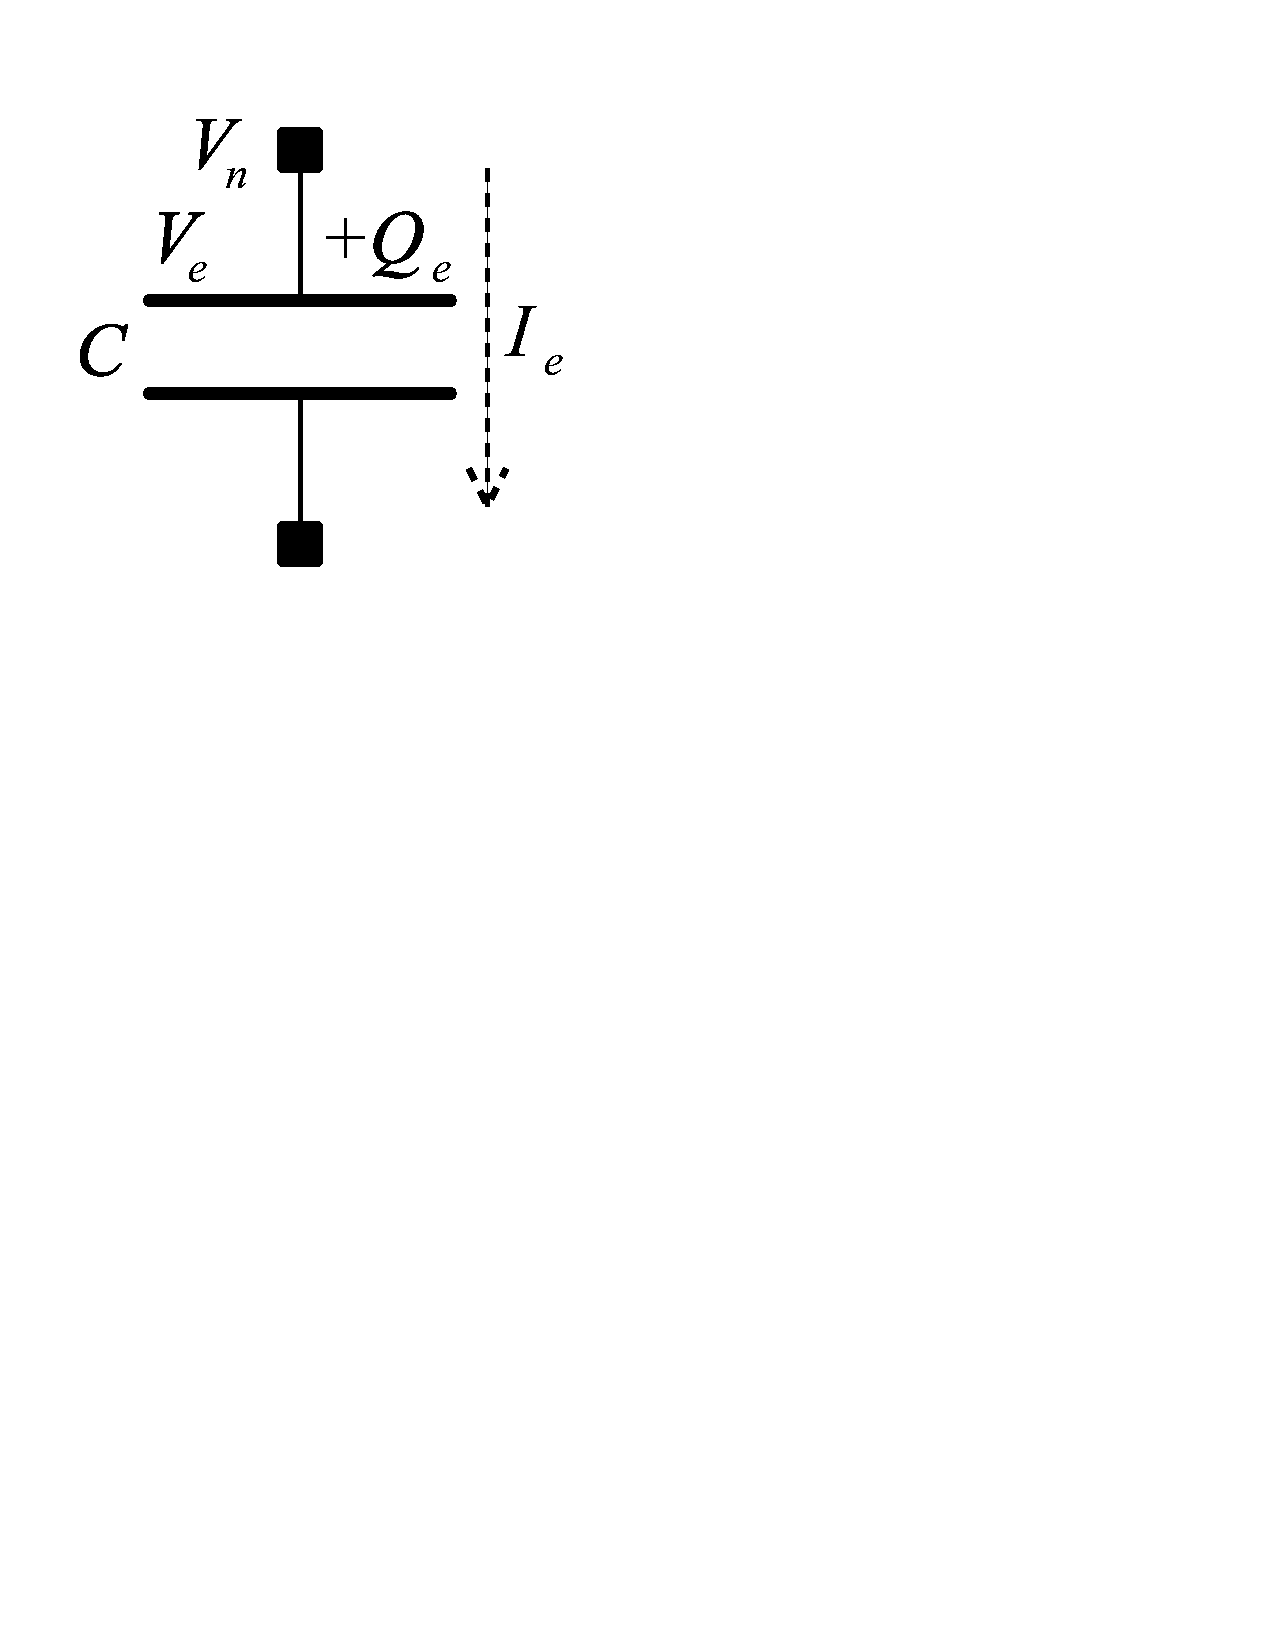
\includegraphics[trim = 0in 7in 4.5in 0in, clip, height=2in]{fig/electrode.pdf}
  \caption{Electrode element}
  \label{fig:Electrode_Element}
\end{figure}
The equation governing this element is,
\begin{eqnarray}
Q_e &=& C_e V_e
\end{eqnarray}
The matrix representation becomes,
\begin{eqnarray}
\left[
\begin{array}{ccc}
0 & 0 & \mathtt{lt}  \\
0 & 0 & 0  \\
0 & 0 & 0  \\
\end{array}
\right]
\left[
\begin{array}{c}
\dot{V}_n \\
\dot{V}_e \\
\dot{Q}_e
\end{array}
\right]
+
\left[
\begin{array}{rrr}
0  &  0 & 0  \\
0  &  0 &-1  \\
1  & -1 & 0
\end{array}
\right]
\left[
\begin{array}{c}
{V}_n \\
{V}_e \\
{Q}_e
\end{array}
\right]
=
\left[
\begin{array}{c}
0 \\
0 \\
0
\end{array}
\right]
\end{eqnarray}
$V_n$ represents the voltage variable at the node which
is linked to the finite element mesh. Two element variables
are introduced, $V_e$ and $Q_e$. 
$V_e$, which is additionally a global variable, is introduced 
to tie the selected
potentials of the finite element mesh to one variable. 
This global variable is then linked to $V_n$. Thus a 
shape function for the global variable must  be specified
for the formulation. $Q_e$ represents the total charge on 
the plate. 

The classes provides the following constructors:
\begin{codelist}

  \item[Electrode(vglobalid)] Creates an Electrode element 
  with \ttt{vglobalid}.

  \item[Electrode2(vglobalid)] Creates an Electrode element 
  with \ttt{vglobalid}.

\end{codelist}

